\documentclass[border=8pt]{standalone}
\usepackage{fontspec}\usepackage{tikz}
\usetikzlibrary{arrows.meta,positioning}
\definecolor{NouOrange}{HTML}{FA4D1F}\definecolor{NouBlack}{HTML}{000000}
\begin{document}
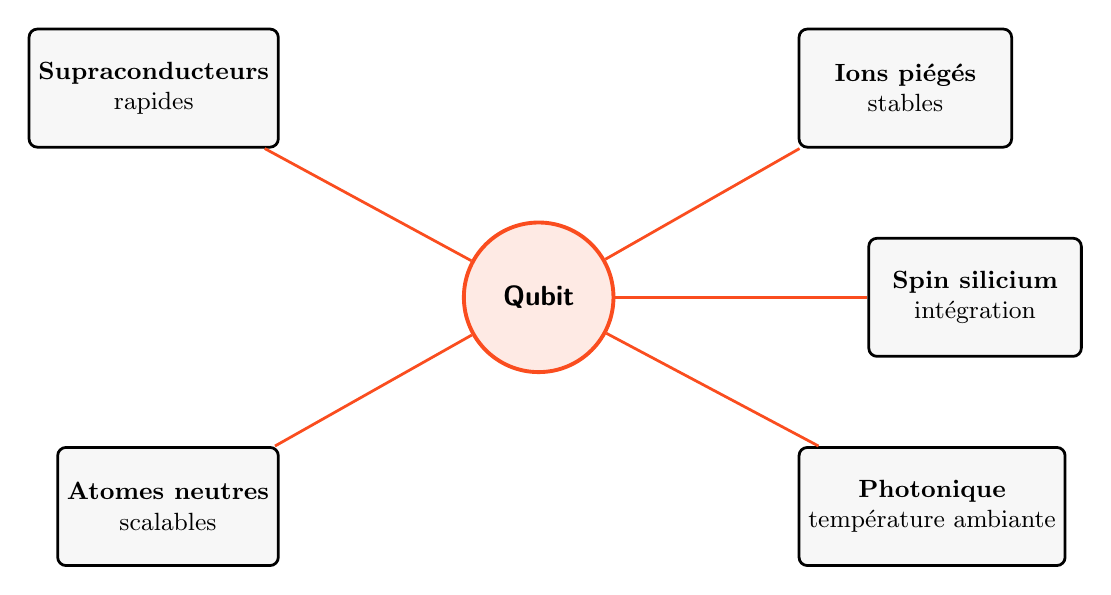
\begin{tikzpicture}[font=\sffamily,
  fam/.style={draw=NouBlack,line width=1pt,rounded corners=3pt,align=center,minimum width=2.7cm,minimum height=1.5cm,fill=black!3,font=\small}]
  \node[draw=NouOrange,line width=1.4pt,circle,fill=NouOrange!12,minimum size=1.9cm,align=center] (c) {\textbf{Qubit}};
  \node[fam,above left=1.2cm and 2.6cm of c] (s) {\textbf{Supraconducteurs}\\rapides};
  \node[fam,above right=1.2cm and 2.6cm of c] (i) {\textbf{Ions piégés}\\stables};
  \node[fam,below left=1.2cm and 2.6cm of c] (a) {\textbf{Atomes neutres}\\scalables};
  \node[fam,below right=1.2cm and 2.6cm of c] (p) {\textbf{Photonique}\\température ambiante};
  \node[fam,right=3.2cm of c] (si) {\textbf{Spin silicium}\\intégration};
  \foreach \n in {s,i,a,p,si}{\draw[NouOrange,line width=1pt] (c) -- (\n);}
\end{tikzpicture}
\end{document}
